\documentclass[10pt,journal]{IEEEtran}
% Add the compsocconf option for Computer Society conferences.
\usepackage{mathtools}
\usepackage{amssymb,amsmath}
\usepackage[T1]{fontenc}
\usepackage{ifpdf}
\usepackage{url}
\ifpdf
\usepackage[pdftex]{graphicx}
\graphicspath{{figs/}}
\DeclareGraphicsExtensions{.pdf,.png,.jpg}
\else
\usepackage[dvips]{graphicx}

\graphicspath{{eps/}}
\DeclareGraphicsExtensions{.eps}
\fi
\usepackage{float}
%\usepackage[caption=false,font=footnotesize]{subfig}
\usepackage[font=footnotesize]{caption}
\usepackage{subcaption}
\usepackage{setspace}
\usepackage{balance}
\pdfminorversion=6
\hyphenation{op-tical net-works semi-conduc-tor}
\newcommand{\indentitem}{\setlength\itemindent{0pt}}
\usepackage{algorithmic}
\usepackage{algorithm}
\newcommand{\algorithmicinput}{\textbf{Input:}}
\newcommand{\INPUT}{\item[\algorithmicinput]}
\newcommand{\algorithmicoutput}{\textbf{Output:}}
\newcommand{\OUTPUT}{\item[\algorithmicoutput]}
\renewcommand{\algorithmicrequire}{\textbf{Pre Condition:}}
\renewcommand{\algorithmicensure}{\textbf{Post Condition:}}
\floatname{algorithm}{Procedure}
\usepackage{tikz}
\usetikzlibrary{matrix,arrows,circuits.ee,circuits.ee.IEC,shapes.geometric,shapes.misc}
\newcommand{\iap}{\textit{DREMS}}
%\newcommand{\iapfull}{\textbf{D}istributed \textbf{S}oftware \textbf{P}latform }
\newcommand{\iapfull}{\textbf{D}istributed \textbf{RE}altime \textbf{M}anaged \textbf{S}ystem}% Algorithmic modifications
\newcommand{\ALOOP}[1]{\ALC@it\algorithmicloop\ #1%
  \begin{ALC@loop}}
\newcommand{\ENDALOOP}{\end{ALC@loop}\ALC@it\algorithmicendloop}
\renewcommand{\algorithmicrequire}{\textbf{Input:}}
\renewcommand{\algorithmicensure}{\textbf{Output:}}
\newcommand{\algorithmicbreak}{\textbf{break}}
\newcommand{\BREAK}{\STATE \algorithmicbreak}
\newenvironment{noindlist}
 {\begin{list}{\labelitemi}{\leftmargin=0.1em \itemindent=0em \itemsep=0.3em}}
 {\end{list}}
\usepackage{multirow}

\begin{document}
\title{ DREMS-OS: An Operating System for Managed Distributed Real-time Embedded Systems }
\vspace{-0.1in}
\author{\IEEEauthorblockN{Abhishek Dubey, Gabor Karsai, Aniruddha Gokhale, William Emfinger, Pranav Kumar\\} 
\IEEEauthorblockA{
  ISIS, Dept of EECS, Vanderbilt University, Nashville, TN 37235, USA \\
 % Email:\{tbd@isis.vanderbilt.edu\}
}
}

% make the title area

%\setcounter{page}{1}
\maketitle
\begin{abstract}
\label{sec:abstract}

%% 1. what is the problem 
Scientific applications that run on leadership computing facilities often face the challenge 
of being unable to fit leading science cases onto accelerator devices due to memory constraints 
(memory-bound applications).
%
% 2. what is your solution 
In this work, the authors studied one such US Department of Energy mission-critical condensed matter 
physics application, Dynamical Cluster Approximation (DCA++), and this paper discusses how device memory-bound challenges were successfully reduced  by proposing an effective 
``all-to-all'' communication method---a ring communication algorithm. 
%
This implementation takes advantage of acceleration on GPUs and remote direct memory access (RDMA) for fast data exchange between GPUs. 
%
\\Additionally, the ring algorithm was optimized with sub-ring communicators
and multi-threaded support to further reduce communication overhead and 
expose more concurrency, respectively.
%
% 3. What's the cherry-picked evaluation result you want to mention
The computation and communication were also analyzed 
by using the Autonomic Performance Environment for Exascale 
(APEX) profiling tool,  and this paper further discusses the 
performance trade-off for the ring algorithm implementation. 
%
The memory analysis on the ring algorithm shows that the allocation size for the authors' most 
memory-intensive data structure per GPU is now reduced to $1/p$ of the original size, where $p$ is the number of GPUs in the ring communicator.
%
The communication analysis suggests that 
the distributed Quantum Monte Carlo execution time grows linearly as sub-ring size increases, and the cost of messages passing through the network interface connector could be a limiting factor.


%
% \todoRed{Ronnie: Next sentence needs rewrite, too much information about Green's function that no one knows in the abstract; recommend generalizing.} \emph {However, DCA++ is currently facing memory-bound challenge as 
% a larger device array $G_t$ is limited by device memory size, where
% $G_t$ is a two-particle Green's function that allows condensed matter
% scientists to explore larger and more complex (higher fidelity)
% physics cases.}

\end{abstract}

\keywords{DCA++, Quantum Monte Carlo, GPU Remote Direct Memory Access, memory-bound issue, exascale machines}


Reinforcement learning has achieved great success in areas such as Game-playing \citep{silver2018general,vinyals2019grandmaster}, robotics \cite{kober2013reinforcement}, large language models \citep{ouyang2022training}, etc.
However, due to safety concerns or physical limitations, in some real-world reinforcement learning problems, we must consider additional constraints that may influence the optimal policy and the learning process \citep{garcia2015comprehensive}.
% For example, a robotic arm must not take actions that may cause harm to itself or the environments.
A standard framework to handle such cases is the constrained Markov Decision Process (CMDP) \citep{altman1999constrained}.
Within the CMDP framework, the agent has to maximize
the expected cumulative reward while
obeying a finite number of constraints, which are usually in the form of expected cumulative cost criteria.

However, we are sometimes concerned with the problem with a continuum of constraints.
For example,
the constraints we meet might be time-evolving or subject to uncertain parameters, which
cannot be formulated as an ordinary CMDP
(see Examples \ref{Example_Time_Evolving} and  \ref{Example_Uncertain}).
In this paper we would study a generalized CMDP  
to address the above problem.  Because the constraints are not only infinite-number but also lie
in a continuous set,
the generalization is not trivial. Fortunately, we find that we can borrow the idea behind semi-infinite programming (SIP) \citep{remez1934determination, hettich1993semi} to deal with the semi-infinite constraints.
Accordingly, we propose \emph{semi-infinitely constrained Markov decision processes} (SICMDPs)
as a novel complement to the ordinary CMDP framework.
%More specifically,  an SICMDP model %, we consider 
%contains a continuum of constraints whereas an ordinary CMDP contains a finite number of constraints. 

%This generalization is natural but not trivial. However, we can brows the idea  
%The idea is quite natural and can be backtracked
%to the practice of extending linear programming to linear semi-infinite programming (LSIP) %\cite{remez1934determination, GobernaLSIO1998}.
%In addition, 
%As a complementary approach to the ordinary CMDP framework, 
%SICMDP can be used to model these problems  which cannot be described by a finite number of constraints
%that are not covered by .
%For example,
%the restrictions we consider can be time-evolving or subject to uncertain parameters
%, thus
%cannot be described by a finite number of constraints but a continuum of constraints 
%(see Examples \ref{Example_Time_Evolving} and  \ref{Example_Uncertain}).

We also present two reinforcement learning algorithms to solve SICMDPs called SI-CRL and SI-CPO, respectively.
SI-CRL is a model-based reinforcement learning algorithm designed for tabular cases, and SI-CPO is a policy optimization algorithm for non-tabular cases.
% and analyze its performance both theoretically and empirically.
The main challenge is that we need to deal with a continuum of constraints, thus reinforcement learning algorithms for ordinary CMDPs do not work anymore.
In SI-CRL, we tackle this difficulty by first transforming the reinforcement learning problem to an equivalent LSIP problem, which can then be solved using methods in the LSIP literature like the dual exchange methods \citep{Hu1990,reemtsen1998numerical}.
In SI-CPO, we resort to the idea of cooperative stochastic approximation developed in \cite{lan2020algorithms, wei2020comirror}.
As far as we know, we are the first to introduce tools from semi-infinitely programming (SIP) into the reinforcement learning community for solving constrained reinforcement learning problems.

% To the best of our knowledge, we are the first to apply tools from semi-infinitely programming (SIP) to solve reinforcement learning problems.
Furthermore, we give theoretical analysis for both SI-CRL and SI-CPO.
We decompose the error of SI-CRL into two parts: the statistical error from approximating the true SICMDP with an offline dataset and the optimization error due to the fact that the solution of the LSIP problem obtained by the dual exchange method is inexact.
On the optimization side, we show that the iteration complexity of SI-CRL is $O\left(\left\{\mathrm{diam}(Y)L\sqrt{|\gS|^2|\gA|m}/\left[(1-\gamma)\epsilon\right]\right\}^m\right)$.
On the statistical side, we show that the sample complexity of SI-CRL is $\widetilde O\left(\frac{|S|^2|A|^2}{\epsilon^2(1-\gamma)^3}\right)$ if the offline dataset is generated by a generative model, and $\widetilde O\left(\frac{|S||A|}{\nu_{\min} \epsilon^2(1-\gamma)^3}\right)$ if the dataset is generated by a probability measure $\nu$ as considered in \cite{chen2019information}.
Here $\widetilde O$ means that all logarithm terms are discarded.
For SI-CPO, things become a little more complicated because other than the statistical error and the optimization error, we also need to consider the function approximation error, which comes from imperfect policy parametrizations.
It is shown if the function approximation error can be controlled to $O(\epsilon)$ order, the iteration complexity of SI-CPO is $\widetilde{O}\left(\frac{1}{\epsilon^2(1-\gamma)^6}\right)$ and the sample complexity of SI-CPO is $\widetilde{O}(\frac{1}{\epsilon^4(1-\gamma)^{10}})$.
Here our iteration complexity bound is equivalent to a typical $\widetilde O(1/\sqrt{T})$ global convergence rate.

We perform a set of numerical experiments to illustrate the SICMDP model and validate our proposed algorithms.
Specifically, we examine two numerical examples, namely the discharge of sewage and ship route planning.
Through the discharge of sewage example, we show the advantage of the SICMDP framework over the CMDP baseline obtained by naive discretization in modeling realistic sequential decision-making problems.
Moreover, we demonstrate the effectiveness of the SI-CRL and SI-CPO algorithms in such tabular environments. 
In the ship route planning example, we illustrate the benefits of the SICMDP framework and the ability of the SI-CPO algorithm to address complex continuous control tasks involving continuous state spaces with modern deep reinforcement learning techniques.

% In summary, our contributions are listed as follows.
% First, we present the SICMDP model, which can be viewed as a generalization of the ordinary CMDP model.
% Second, we propose an algorithm to perform reinforcement learning for SICMDPs, which is called SI-CRL, and we believe that we are the first to apply tools from SIP
% to solve reinforcement learning problems.
% Third, we give a theoretical analysis of SI-CRL and identify both its sample complexity and iteration complexity.
% In addition, we perform numerical experiments to illustrate the SICMDP model and validate the SI-CRL algorithm.
% \{This paragraph can be removed!!! \}






\section{Related Work}
\label{sec: Related Work}
In this section, we introduce two representative diversity estimators and discuss the difficulties they meet when handling MMOPs. Subsequently, some existing multi-modal multi-objective optimization algorithms are reviewed.
\subsection{Review of diversity estimators}
\subsubsection{Density in SPEA2}
In SPEA2 \cite{SPEA2}, each solution is assigned a density value which is used to calculate its fitness value. Eq. (\ref{eq: Density in SPEA2}) gives the density of a solution $\boldsymbol{x}$.
\begin{equation}
	\textit{Density} (\boldsymbol{x}) = \frac{1}{\sigma_k(\boldsymbol{x}) + 2},
	\label{eq: Density in SPEA2}
\end{equation}
where $\sigma_k(\boldsymbol{x})$ is the distance from $\boldsymbol{x}$ to its $k$-th nearest neighbor in the objective space. In SPEA2, $k$ is set to the square root of the total number of solutions in the current population as a general parameter setting.

Notice that in SPEA2, higher density means worse diversity in the objective space.

\subsubsection{Crowding distance}
Crowding distance is proposed along with the NSGA-II algorithm\cite{NSGAII} to preserve the diversity of the population in the objective space. The crowding distance of a solution $\boldsymbol{x}$ is given by the average side length of the hypercube constructed by its left and right neighbors in each objective. More precisely, for each objective, the left and right neighbors of $\boldsymbol{x}$ are the solutions at the left and right positions of $\boldsymbol{x}$ for that objective (i.e., in the list obtained by sorting the population in an increasing order of the objective values of that objective). The crowding distance of all boundary solutions (i.e., best solutions in any objectives) are set to $\infty$ to ensure that they are always selected. In NSGA-II, larger crowding distance values indicate better diversity. Formally, Eq. (\ref{eq: crowding distance}) calculates the crowding distance for a solution $\boldsymbol{x}$.
\begin{equation}
	\textit{Crowding-Distance} (\boldsymbol{x}) =
	\begin{cases}
		\infty                                                                     & ,\boldsymbol{x} \text{ is a boundary solution} \\
		\frac{1}{M}\sum_{m=1}^M[f_m(\boldsymbol{x}_{rm})-f_m(\boldsymbol{x}_{lm})] & ,\text{otherwise}
	\end{cases},
	\label{eq: crowding distance}
\end{equation}
where $M$ refers to the number of objectives, and $\boldsymbol{x}_{lm}$ and $\boldsymbol{x}_{rm}$ are the left and right neighbors of solution $\boldsymbol{x}$ regarding the $m$-th objective, respectively.
\subsection{Difficulties when handling MMOPs}
In most diversity estimators in MOEAs, the solution distribution in the decision space is out of consideration, which makes them inefficient on MMOPs. As we have discussed in Section \ref{sec: Introduction}, in MMOPs, equivalent solutions have the same or almost the same objective values. Consequently, they are usually not preferable in terms of diversity (in the objective space). For this reason, diversity estimators used in MOEAs are often responsible for the loss of equivalent solutions when tackling MMOPs. Fig. \ref{fig: Difficulty when handling MMOPs} gives an example when a diversity estimator such as crowding distance produces undesirable effects. In Fig. \ref{fig: Difficulty when handling MMOPs}, $A$ and $B$ are two Pareto optimal solutions on different (but equivalent) Pareto subsets (i.e., the upper and lower dash lines in (a)). Although $A$ and $B$ have similar objective values, the decision maker may want to keep both of them since they represent different implementations (i.e., they are different in the decision space). However, a diversity estimator tends to assign bad diversity values to them due to the small difference between their objective values. As a result, some of them are likely to be removed. From this example, we can see that solutions in different regions in the decision space should be considered separately when estimating solution diversity for MMOPs. Following this idea, we propose a niching diversity estimation method in Section \ref{sec: Proposed method}.

\begin{figure}
	\centering
	\includegraphics[width=.75\textwidth]{figures/RelatedWork/Difficulties}
	\caption{Explanation of the diversity loss in the decision space caused by diversity estimators when handling an MMOP. The dash lines in (a) and (b) denote the Pareto set and Pareto front, respectively.}
	\label{fig: Difficulty when handling MMOPs}
\end{figure}

\subsection{Multi-modal multi-objective optimization algorithms}
\label{sec: Existing multi-modal multi-objective optimization algorithms}
In most state-of-the-art multi-modal multi-objective evolutionary algorithms (MMEAs), the diversity in the decision space is maintained by niching strategies. Some MMEAs extend existing niching strategies in MOEAs to enable them to maintain the diversity in the objective space as well as in the decision space. For example, in \cite{OmniOptimizer}, Deb and Tiwari proposed one of the first MMEA called Omni-optimizer which modifies the crowding distance to measure the diversity in the decision space and the objective space simultaneously. Yue et. al. proposed a particle swarm optimizer named MO\_Ring\_PSO\_SCD \cite{MO_Ring_PSO_SCD} which adopts a similar modified crowding distance and a ring topology to create a niche structure. The DNEA algorithm \cite{DNEA} applies the fitness sharing \cite{Sharing} to both decision and objective spaces and combines them into a single sharing function. Some MMEAs are proposed with dedicated niching strategies in the decision space. Tanabe et. al. proposed a decomposition-based MMEA called MOEA/D-AD\cite{MOEAD_AD} where multiple solutions can be assigned to a weight vector, and a newly generated solution only competes with other solutions which are assigned to the same weight vector and neighboring to that solution in the decision space. In our previous study \cite{MOEAD_MM}, we proposed another decomposition-based MMEA which utilizes a clearing strategy in the decision space. Some MMEAs such as the algorithms proposed in \cite{DBSCAN_MMEA} and \cite{MMOEADC} use clustering approaches to maintain the niching structure in the decision space.

% $Id: taskModel.tex 3909 2013-10-22 06:07:02Z dabhishe $
\vspace{-0.09in}
\section{DREMS Architecture}
\label{sec:task_model}
% This section provides background material and states assumptions for the rest of the paper. 
% in this paper. 
% We also describe the underlying
%system model used for our research.
%\vspace{-0.05in}
%\subsection{\iap\ Architecture}
\iap\ \cite{ISIS_F6_Aerospace:12,6899124,4813} is a distributed system architecture that consists
of one or more computing nodes grouped into a cluster. It is conceptually similar to the recent Fog Computing Architecture \cite{vaquero2014finding}. Distributed applications, composed from cooperating
processes called \textit{actors}, provide services for the end-user.
Actors specialize the notion of OS processes; 
they have persistent identity that allows them to be transparently
migrated between nodes, and they have strict limits on resources that
they can use.  Each actor is constructed from one or more reusable
components~\cite{ISIS_F6_ISORC:13,4813} where each component is
single-threaded.  
% Abhishek, commenting this out.
% Recently, this architecture has been extended to create  applications for smart grid \cite{4813}. 

% \vspace{-0.05in}
% \subsection{The Linux Scheduler}
% \label{sec:linuxScheduler}
% The \iap\ OS scheduler builts upon the standard Linux scheduler
% (kernel version: 3.2.7).  The scheduler is responsible for allocating
% CPU resource(s) to all currently running computational entities.
% Schedulers are implemented in the Linux kernel through \emph{scheduler
%   classes}.  The two important scheduler classes are CFS (Completely Fair
% Scheduler) and the RT (Real Time) scheduler~\cite{mauerer2008}.
% The CFS scheduler attempts to allocate CPU time between processes
% fairly, while the RT scheduler selects processes based on their priority. 

% Tasks eligible for scheduling are maintained in a structure called the
% \emph{runqueue}. Each CPU core has its own runqueue. However
% the runqueue is not necessarily just a queue: it consists of a 
% %-- it is a container using a data structure that contains 
% a bit array,  with one bit for each priority level and a list containing the 
% tasks ready to be scheduled at that level.
% The bit at a level is set to one when there are tasks at that level.
% A 0 value indicates an empty queue at that level. In a multi core
% system, this structure is replicated per CPU. In a fully preemptive
% mode, the scheduling decision is made by  evaluating which task should be
% executed next on a CPU when an interrupt handler exits, when a 
% system call returns, or when the scheduler function is
% explicitly invoked to preempt the current process.

%\begin{figure}[t]
%\centering
%\includegraphics[width=0.45\textwidth]{runqueue}
%\caption{Scheduler Runqueues}
%\label{fig:runqueue}
%\end{figure}

\iffalse
Next sections describe the \iap\ Scheduler features and their main
algorithms. This scheduler was implemented by changing the behavior of
the linux scheduler described in this subsection.  
\fi
\vspace{-0.05in}
%\subsection{Spatial and Temporal Partitioning}
%\label{sec:tasks}

\iffalse
While most tasks\footnote{We use the term threads and tasks
  interchangeably in this paper.} perform application functions,
some tasks are used for system management and mission-critical functions.  
Thus, we group these tasks into different criticality levels: (a) 
\emph{Critical} tasks are those tasks which are required
for system and mission management; (b)
\emph{Application} tasks perform mission-specific, non-critical work; 
(c)
%\emph{System Management}[kernel] tasks provide the interfaces to the
%kernel resources and can be configured to have a fixed percentage of
%CPU time reserved for these tasks; and finally (d)
 \emph{Best Effort}
tasks are those low priority tasks that are scheduled only when there
are no runnable tasks from the previous two categories.
\fi 
\begin{figure}[t]
\centering
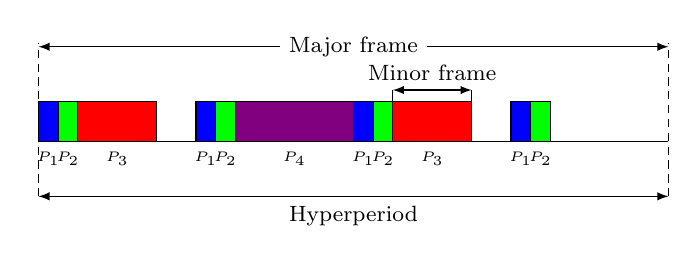
\begin{tikzpicture}[x=1cm,y=1cm, 
every label/.style={font=\tiny},
p1/.style={shape=rectangle,draw,fill=blue, align=center,font=\tiny,minimum height=5mm,minimum width=2.5mm},
p2/.style={shape=rectangle,draw,fill=green,align=center,font=\tiny,minimum height=5mm,minimum width=2.5mm},
p3/.style={shape=rectangle,draw,fill=red,  align=center,font=\tiny,minimum height=5mm,minimum width=10mm},
p4/.style={shape=rectangle,draw,fill=red!50!blue,align=center,font=\tiny,minimum height=5mm,minimum width=15mm},
]
\def\pdist{0.25}\def\hpy{-.95}\def\MF{.95}\def\mfh{.4}\def\mfbeg{17.5*\pdist}\def\mfend{21.5*\pdist}\def\labelpos{270}
\node[p1](P11) at (   0*\pdist,0) [label=\labelpos:$P_1$]{}; \node[p2](P21) at ( 1*\pdist,0) [label=\labelpos:$P_2$] {};
\node[p3](P31) at ( 3.5*\pdist,0) [label=\labelpos:$P_3$]{}; 
\node[p1](P12) at (   8*\pdist,0) [label=\labelpos:$P_1$]{}; \node[p2](P22) at ( 9*\pdist,0) [label=\labelpos:$P_2$] {};
\node[p4](P41) at (12.5*\pdist,0) [label=\labelpos:$P_4$]{}; 
\node[p1](P13) at (  16*\pdist,0) [label=\labelpos:$P_1$]{}; \node[p2](P23) at (17*\pdist,0) [label=\labelpos:$P_2$] {};
\node[p3](P32) at (19.5*\pdist,0) [label=\labelpos:$P_3$]{};
\node[p1](P14) at (  24*\pdist,0) [label=\labelpos:$P_1$]{}; \node[p2](P24) at (25*\pdist,0) [label=\labelpos:$P_2$] {};
\draw[densely dashed,-] (-0.5*\pdist,\hpy) -- (-0.5*\pdist,1); \draw[densely dashed,-] (31.5*\pdist,\hpy) -- (31.5*\pdist,1);
\draw[-] (-0.5*\pdist,-.25) -- (31.5*\pdist,-.25);
\draw[latex-latex] (-0.5*\pdist,\hpy) -- (31.5*\pdist,\hpy) node [below,align=center,midway,font=\footnotesize] {Hyperperiod};
\draw[latex-latex] (-0.5*\pdist,\MF) -- node[sloped,fill=white,font=\footnotesize]{Major frame} (31.5*\pdist,\MF);
%
\draw[-] (\mfbeg,0) -- (\mfbeg,\mfh); \draw[-] (\mfend,0) -- (\mfend,\mfh);
\draw[latex-latex] (\mfbeg,\mfh) -- (\mfend,\mfh) node [above,align=center,midway,font=\footnotesize] {Minor frame};
\end{tikzpicture}%

\caption{A Major Frame. The four partitions (period,duration) in this frame are $P_1$ (2s, 0.25s), $P_2$ (2s, 0.25s), $P_3$ (4s, 1s), and $P_4$ (8s, 1.5s). }
%where the first number is the period and the second number is the duration of the partition.}
\label{fig:validschedule}
\vspace{-0.2in}
\end{figure}

%The length of the repeating frame is also known as the \emph{major frame}.  

%Given a valid schedule as input, the
%scheduler guarantees that actors in separate temporal partitions
%cannot interfere with each other's CPU resource usage.  

%
%
%. For the RT scheduler it is an array combined with bits
%indicating priority. Tasks are added  to the runqueue when they are in ready state and are removed from the runqueue when they are waiting for either a reseource or are sleeping for some time. 
%
%
%
% and removed from the runqueue as they become ready or 
%
%
%The runqueues do not necessarily contain all the
%existing tasks in the system - only those which are eligible for
%scheduling. One example for tasks which are not in any of the queues
%are inactive tasks. When a task becomes inactive it is removed from
%the runqueues (\texttt{dequeue\_task}) and a timer is started. When the
%timer expires, the task is added back to the runqueue
%(\texttt{enqueue\_task}). This dequeuing and enqueing happens each
%time a task changes its state from ready to another state.
%
%When SMP (Symmetric Multiprocessing) is enabled, each CPU manages its own runqueue. Tasks are
%occasionally migrated between CPUs based on a balancing algorithm. The
%RT scheduler runqueue consists of a bitmap and a linked list for each
%priority level. The bitmap contains "1" if the given list contains any
%element - this allows the scheduler to jump to the highest priority 
%ready task in constant time. When a task is added to the list the
%bitmap is updated and the task is added to the linked list belonging
%to the given level. The same steps happen for task removal or a
%change in a task's priority. During a scheduling decision, the
%core scheduler goes through the scheduler classes in their priority
%order and calls the \texttt{pick\_next\_task} function. If it returns with a task, the task will get prioritized. 
%If no task is ready to run, the idle task is scheduled. A 
%scheduling decision happens in one of the following situations:
%
%\begin {itemize}
%\item [A)] When an interrupt handler exits (including the interrupt invoked
%  by the periodic tick timer).
%\item [B)] When a system call returns.
%\item [C)] When the scheduler is invoked explicitly by the current running
%  task.
%\end {itemize}

% TODO:  I presume this has yet to be done?
%{\bf describe the preemption-RT patch}



%!TEX root = main.tex
% $Id: f6sched.tex 3898 2013-10-22 04:52:42Z csanad $
%\section{\iap\ OS Scheduler}
%\label{sec:scheduler}
%This section delves into the details of the \iap\ OS scheduler and its
%capabilities.

\subsection{Partitioning Support}
\label{sec:scheduler}
The system guarantees spatial isolation between actors  by (a)
providing  a separate address space for each actor; (b) enforcing that an
I/O device can be accessed by only one actor at a time; and (c)
facilitating temporal isolation between processes by the scheduler.
Spatial isolation is implemented by the Memory Management Unit of the CPU,  
while temporal isolation is provided via ARINC-653~\cite{ARINC-653} style
\textit{temporal partitions}, implemented in the OS scheduler. 

%-- a periodically repeating fixed interval of the CPU's time exclusively assigned to a group of 
% cooperating actors of the same  application. 
% Abhishek, in the intro we have mentioned limitations with such a
% partitioning scheme and cited the very same reference. So here we need
% to say a sentence saying that there is a slight difference as
% explained in Section~\ref{sec:scheduler}.

A temporal partition is characterized by two parameters: period and
duration.  The period reflects how often the tasks of the
partition will be guaranteed CPU allocation.  The duration governs the
length of the CPU allocation window in each cycle.  Given the period
and duration of all temporal partitions, an execution schedule can be
generated by solving a series of constraints, see~\cite {ACM_SPE:10}.
A feasible solution, \emph{e.g.} Figure~\ref{fig:validschedule}, comprises
a repeating frame of windows, where each window is assigned to a
partition.  These windows are called \emph{minor frames}.  The length
of a window assigned to a partition is always the same as the duration
of that partition.  The repeating frame of minor frames, known as the \emph{major frame},
has a length called the \emph{hyperperiod}.  The hyperperiod is the lowest common multiple
of the partition periods.  


\subsection{Criticality Levels Supported by the \iap\ OS Scheduler}
\label{sec:criticality_levels}
The \iap\ OS scheduler can manage CPU's time
for tasks on three different criticality levels:
\emph{Critical}, \emph{Application} and \emph{Best Effort}.
The \emph{Critical} tasks provide kernel level services and system
management services. These tasks will be scheduled based on their
priority whenever they are ready. \emph{Application} tasks are
mission specific and are isolated from each other. These tasks are
constrained by temporal partitioning and can be preempted by tasks of the
\emph{Critical} level. Finally, \emph{Best Effort} tasks are executed
whenever no tasks of any higher criticality level are available.

Note that actors in an application can have different criticality levels,
but all tasks associated with an actor must have the same criticality
level, \emph{i.e.} an actor cannot have both \emph{Critical} tasks and
\emph{Application} tasks.

\subsection{Multiple partitions}
\label{sec:datastructure}
To support the different levels of criticality, we extend the \textit{runqueue} data structure of the Linux kernel \cite{garg2009real}. A runqueue maintains a list of tasks eligible for scheduling. %It consists of a bit array with one bit for each priority level and a list containing the tasks ready to be scheduled at that level. The bit at a level is set to one when there are tasks at that level, a 0 value indicates an empty queue at that level. 
In a multicore system, this structure is replicated per CPU. In a fully preemptive mode, the scheduling decision is made by  evaluating which task should be executed next on a CPU when an interrupt handler exits, when a system call returns, or when the scheduler function is explicitly invoked to preempt the current process.
We created one runqueue per temporal partition per CPU. Currently, the system can support 64 {\it Temporal partitions}, also referred to as Application partitions in the sequel. One extra runqueue is created for the critical tasks. These tasks are said to belong to the {\it System partition}.  The Best effort tasks are managed through the Linux Completely Fair Scheduler (default) runqueue and are considered for execution as part of the System partition when no other tasks are eligible to run. 



\subsection{CPU Cap and Work Conserving Behavior}
\label{sec:CPUCAP}
The schedulability of the \emph{Application} level tasks is
constrained by the current load coming from the \emph{Critical} tasks
and the temporal partitioning used on the \emph{Application} level.
Should the load of the \emph{Critical} tasks exceed a threshold the system
will not be able to schedule tasks on the \emph{Application} level. A
formal analysis of the response-time of the \emph{Application} level
tasks will not be provided in this paper, however, we present a 
description of the method we will use to address the analysis which
will build on available results from
\cite{BaruahRTA4MCS, PartitionedRTA-Almeida04, 
HierarchicalRTA-Lipari05}.

The submitted load function $H_i(t)$ determines the maximum load
submitted to a partition by the task $\tau_i$ itself after its
release together with all higher priority tasks belonging to
the same partition. The availability function $A_S(t)$ returns for
each time instant the cumulative computation time available for the
partition to execute tasks. In the original model~\cite{PartitionedRTA-Almeida04}
$A_S(t)$ is the availability function of a periodic server.
 The response-time of a task $\tau_i$ is the time
when $H_i(t)$ intersects the availability function $A_S(t)$ for the
first time.  In our system $A_S(t)$ is decreased by the load of the
available \emph{Critical} tasks which, if unbounded, could block the
application level tasks forever. This motivates us to enforce a bound
on the load of the \emph{Critical} tasks. This bound is referred to as
{\bf CPU cap}.
% It is our future goal to come up with a bound backed by a theoretical analysis.

In \iap\ OS, the CPU cap can be applied to tasks on the
\emph{Critical} and \emph{Application} level to provide scheduling
fairness within a partition or hyperperiod. Between criticality
levels, the CPU cap provides the ability to prevent higher
criticality tasks from starving lower criticality tasks of the CPU.
On the \emph{Application} level, the CPU cap can be used to bound
the CPU consumption of higher priority tasks to allow the execution
of lower priority tasks inside the same partition. If the CPU cap
enforcement is enabled, then it is possible to set a maximum CPU
time that a task can use, measured over a configurable number of
major frame cycles.

%In addition to partition scheduling, each application task or system task can have a
%CPU cap resource assigned to it to provide scheduling fairness within
%a partition or hyperperiod, if the CPU cap enforcement is enabled.  The CPU cap
%provides the ability to prevent high priority application tasks from
%starving lower priority tasks of the CPU.
%The enforcement of the CPU cap is work conserving within partitions. 

%For application tasks which share a temporal partition, the scheduler
%provides a work conserving ceiling on each task's utilization of the
%CPU. This ceiling, the CPU cap, restricts the task to a percentage of
%time on the CPU over a configurable period.  Tasks which share a
%partition are scheduled in a work conserving manner, \emph{i.e.} if a
%task has reached its CPU cap but there are no other runnable tasks in
%the partition, the scheduler will continue scheduling the task past
%its ceiling. Additionally, the scheduler allows the temporal
%partitioning schedule to be dynamically updated. Finally, the \iap\
%OS scheduler guarantees that resource over-utilization by a set of
%tasks in one partition will not affect tasks running in another
%partition. Additionally, the scheduler supports a maximum cpu cap
%ceiling that can be imposed on a group of critical level tasks. This
%is necessary to provide a guaranteed CPU time slot to application
%tasks. 

\iffalse
The CPU cap resource for a task is converted into a ceiling of
execution time, which is measured over $N$ major frames. The number
of major frames over which the CPU cap ceiling is calculated is
configurable at compilation time. When CPU cap is enabled, the
scheduler maintains a counter for all tasks. The scheduler also
maintains the current execution time of each task since the start of
the CPU cap window. Note that at the beginning of each CPU cap
window, the execution time of the task is reset to zero whereas the
counter is reset after the number of major frame cycles over which
the cap was specified elapses. 

The counter is used when making a scheduling decision, which requires
consideration of whether a task is ready and whether the task has
surpassed its CPU cap quota.  At every invocation of the scheduler,
the execution time for the task is updated and compared against the
execution time ceiling of the currently running task. If the task
has surpassed its CPU cap quota within the CPU cap window, its
$disabled$ flag is set to $true$.  
%This flag is evaluated for the
%currently running task when the main scheduling function is executed
%and is set when the task reaches its CPU cap.  

%For application tasks which share a temporal partition, the scheduler
%provides a work conserving ceiling on each task's utilization of the
%CPU. This ceiling, the CPU cap, restricts the task to a percentage of
%time on the CPU over a configurable period.  Tasks which share a
%partition are scheduled in a work conserving manner, \emph{i.e.} if a
%task has reached its CPU cap but there are no other runnable tasks in
%the partition, the scheduler will continue scheduling the task past
%its ceiling. Additionally, the scheduler allows the temporal
%partitioning schedule to be dynamically updated. Finally, the \iap\
%OS scheduler guarantees that resource over-utilization by a set of
%tasks in one partition will not affect tasks running in another
%partition. Additionally, the scheduler supports a maximum cpu cap
%ceiling that can be imposed on a group of critical level tasks. This
%is necessary to provide a guaranteed CPU time slot to application
%tasks. 
\fi

The CPU cap is enforced in a work conserving manner, \textit{i.e.}, 
if a task has reached its CPU cap but there are no other
available tasks, the scheduler will continue scheduling the task past
its ceiling. In case of \emph{Critical} tasks, when the CPU cap is reached,
the task is not marked ready for execution unless
(a) there is no other ready task in the system; or 
(b) the CPU cap accounting is reset.
This behavior ensures that the kernel tasks, such as those belonging
to network communication, do not
overload the system, for example in a denial-of-service attack.
For the tasks on the \emph{Application} level, the CPU cap is
specified as a percentage of the total duration of the partition,
the number of major frames, and the number of CPU cores
available all multiplied together. When an \emph{Application} task reaches
the CPU cap, it is not eligible to be scheduled again unless 
the following is true: either
(a) there are no \emph{Critical} tasks to schedule and there are no other ready tasks in the partition; or (b) the CPU cap accounting has been reset.

\subsection{Dynamic Major Frame Configuration}
\label{sec:reconfiguration}

\iffalse
This section describes the mechanism used to configure (or reconfigure during a mission) the partition
scheduler, Procedure~\ref{algo:majorframe}.
Table~\ref{table:variable} summarizes the key symbols used in this
and related subsections. 
\begin{table}[ht]
\caption{\iap\ Symbols used in Section \ref{sec:scheduler}}
\footnotesize
\begin{tabular}{| c | p{0.3\textwidth} |}
\hline
 APP\_INACTIVE &The scheduler state in which tasks in temporal partitions are not scheduled \\\hline
 APP\_ACTIVE &Inverse of APP\_INACTIVE\\\hline
$firstrun$& A global variable, set whenever the major frame has been changed\\\hline
$mfl$&A global circular linked list of minor frames used by the scheduler\\\hline
$cur\_frame$&Current minor frame.\\\hline
$HP\_start$&Global variable, stores the start time of a new major frame.\\\hline
\end{tabular}
\label{table:variable}
\end{table}
\fi


%The scheduler states are described in table \ref{table:variable}. Just after boot sequence the scheduler is in  APP\_INACTIVE state. In this state

During the configuration process that can be repeated at
any time without rebooting the node, the kernel receives the major
frame structure that contains a list of minor frames and it also
contains the length of the hyperperiod, partition periodicity, and
duration. Note that major frame reconfiguration can only be
performed by an actor with suitable capabilities.  More details on the
\iap\ capability model can be found in~\cite{ISIS_F6_Aerospace:12}.

Before the frames are set up, the process configuring the frame has to
ensure that the following three constraints are met: (C0) The
hyperperiod must be the least common multiple of partition periods;
(C1) The offset between the major frame start and the first minor
frame of a partition must be less than or equal to the partition
period:  $(\forall p \in \mathbb{P})(O_{1}^{p} \leq \phi(p))$; (C2)
Time between any two executions should be equal to the partition
period: $(\forall p \in
\mathbb{P})(k\in[1,N(p)-1])(O_{k+1}^{p}=O_{k}^{p}+ \phi(p))$, where
$\mathbb{P}$ is the set of all partitions, $N(p)$ is the number of
partitions, $\phi(p)$ is the period of partition $p$ and $\Delta(p)$
is the duration of the partition $p$. $O^p_i$ is the offset of
$i^{th}$ minor frame for partition $p$ from the start of the major
frame, $H$ is the hyperperiod. 

\iffalse
\begin{algorithm}[t]
\caption{Update Major frame}
\label{algo:majorframe}
\begin{algorithmic}[1]
\footnotesize
\INPUT $frame$ \COMMENT{A sorted but not necessarily contiguous major frame structure} 
\REQUIRE $Valid(mf)$
\STATE $Reassign ~Task ~to ~CPU ~0$
\STATE $Acquire~ update~ frame~ spin lock,~ disable~ preemption/interrupts$
\STATE $frame \leftarrow  Fill\_Empty(frame)$ 
\STATE $\bf{Atomic:}$$state \leftarrow  APP\_INACTIVE$
\STATE $ firstrun \leftarrow true$
\STATE $ mfl \leftarrow frame.minorframelist$
\STATE $\bf{Atomic:}$$state \leftarrow  APP\_ACTIVE$
\STATE $Release~ update~ frame~ spin lock,~ enable~ preemption/interrupts$
\end{algorithmic}
\end{algorithm}
\fi
%During configuration of the partition schedule, the scheduler receives a 
%list of minor frames which comprise the schedule.  These minor frames
%are checked against certain constraints, shown below, to verify they
%form a valid schedule. 
%
%\begin{description}
%\item [C0] The start for all partitions must happen before the period ends : $(\forall p \in \mathbb{P})(O_{1}^{p} \leq \phi(p))$.
%\item [C1] The start for all partitions must happen before the period ends : $(\forall p \in \mathbb{P})(O_{1}^{p} \leq \phi(p))$.
%\item [C2] Time between any two executions should be equal to partition period : $(\forall p \in \mathbb{P})(k\in [1,N(p)-1])(O_{k+1}^{p}=O_{k}^{p}+ \phi(p))$.
%\item [C3] The last start must finish before the hyperperiod ends : $(\forall p \in \mathbb{P})(O_{N(p)}^{p}+\Delta(p) \leq H)$
%\item [C4] A partition cannot overlap : $(\forall p \in \mathbb{P})(\forall z \in \mathbb{P})$$(k\in [1,N(p)])(j\in [1,N(z)])$ $(O_{k}^{p} \leq O_{j}^{z} \implies O_{j}^{z} \geq O_{k}^{p} +\Delta(p))$
%\end{description}
%
%
%
% Note that the minor frames need not be contiguous,
%as the algorithm, Procedure~\ref{algo:majorframe}, fills in any gaps 
%automatically.  
%
%Let $\mathbb{P}$ be the set of all partitions in a node. Let $\phi(p) \in \mathbb{R} \cap [0,\infty) $ denote the period of partition $p \in \mathbb{P}$. Let $\Delta(p) \in \mathbb{R} \cap [0,\phi(p)]$ denote the duration of time that a partition needs to be executed every  $\phi(p)$ time units. Then hyperperiod $H$ is given as $H=LCM(\phi(\mathbb{P}))$\footnote{Here  $\phi(\mathbb{P})$ is a used as a succinct  representation of set $\{x|x=\phi(p) \wedge p \in \mathbb{P} \}$. We will use this short representation for other sets also. }, where LCM is the abbreviation for the least common multiple.  The constraints for a valid scheduler are
%
%\begin{description}
%\item [C1] The start for all partitions must happen before the period ends : $(\forall p \in \mathbb{P})(O_{1}^{p} \leq \phi(p))$.
%\item [C2] Time between any two executions should be equal to partition period : $(\forall p \in \mathbb{P})(k\in [1,N(p)-1])(O_{k+1}^{p}=O_{k}^{p}+ \phi(p))$.
%\item [C3] The last start must finish before the hyperperiod ends : $(\forall p \in \mathbb{P})(O_{N(p)}^{p}+\Delta(p) \leq H)$
%\item [C4] A partition cannot overlap : $(\forall p \in \mathbb{P})(\forall z \in \mathbb{P})$$(k\in [1,N(p)])(j\in [1,N(z)])$ $(O_{k}^{p} \leq O_{j}^{z} \implies O_{j}^{z} \geq O_{k}^{p} +\Delta(p))$
%\end{description}

The kernel checks two additional constraints: (1) All minor frames
finish before the end of the hyperperiod: $(\forall i)(O_{i}.start+O_{i}.duration
\leq H)$ and (2) minor frames cannot overlap, i.e. given a sorted minor
frame list (based on their offsets): $(\forall i <
N(O))(O_{i}.start+O_{i}.duration \leq O_{i+1})$, where $N(O)$ is the number
of minor frames.   Note that the minor frames need not be contiguous,
as the update procedure fills in any gaps automatically.

If the constraints are satisfied, then the task is moved to the first core, \emph{CPU0} if it is not already on \emph{CPU0}. 
This is done because the global tick (explained in next subsection) used for implementing the major 
frame schedule is also executed on \emph{CPU0}. By moving the task to \emph{CPU0} and disabling interrupts, 
the scheduler ensures that the current frame is not changed while the major frame is being updated. 
At this point the task also obtains a spin lock to  ensure that no other task can update the major frame at 
the same time. In this procedure the scheduler state is also set to \texttt{APP\_INACTIVE} (see Table \ref{table:variable}), to stop the scheduling of all application
tasks across other cores. The main scheduling loop reads the scheduler state before scheduling application tasks. A  scenario showing dynamic reconfiguration can be seen in Figure~\ref{fig:dynamic_reconfig}. 

\begin{table}[ht]
\centering
\caption{The states of the DREMS Scheduler}
\footnotesize
\begin{tabular}{| c | p{0.3\textwidth} |}
\hline
 APP\_INACTIVE &Tasks in temporal partitions are not run \\\hline
 APP\_ACTIVE &Inverse of APP\_INACTIVE\\\hline
\end{tabular}
\label{table:variable}
\end{table}

\iffalse
the scheduler state is set to
\texttt{APP\_INACTIVE}, to stop the scheduling of all application
tasks so the partition structure can be updated.  Note that while the
scheduler state is set to \texttt{APP\_INACTIVE}, the $mfl$ in
Procedure~\ref{algo:globaltick} will be $null$, so the partition
scheduling will be halted.   The scheduler state is set to
\texttt{APP\_ACTIVE} to begin scheduling these application tasks per
the schedule.   
To ensure that multiple processes cannot try to change the partition
schedule at the same time, Procedure~\ref{algo:majorframe} uses a 
spinlock to ensure that multiple processors cannot execute this code 
simultaneously.  Additionally, all other processors except for \emph{CPU0} only
ever atomically read the major frame structure to ensure data structure consistency.
\fi

%Why is the important to have synchronized hyper periohd.
%parts of the same application are distributed across the node.
% low latency communication.
%Every node will run the related tasks at the same time.
%Note that, though it is not shown in the algorithm, 

It is also possible to set the global tick (that counts the hyperperiods) to be started with an offset. 
This delay can be used to synchronize the start of the hyperperiods across nodes of the cluster. This is necessary to 
ensure that all nodes schedule related temporal partitions at the same time.
%The activation of this schedule can be set to occur at a specific
%time, so the partition schedules on multiple computing nodes can be
%synchronized.
This ensures that for an application that is distributed
across multiple nodes, its \emph{Application} level tasks run at
approximately the same time on all the nodes which enables low latency
communication between dependent tasks across the node level. 

%Unlike many temporally partitioned schedulers, \iap\ OS provides
%functionality for dynamic reconfiguration of the temporal partition
%schedule.  This capability allows the system to switch between scenarios
%while running.  The dynamic reconfiguration is achieved by atomically
%setting the scheduler state to \texttt{APP\_INACTIVE}, which stops all
%application actors contained within partitions from being scheduled.
%While in this state, a new schedule can be loaded through system calls
%during run-time.  Once updated, the new partition schedule can be
%started by changing the scheduler state back to \texttt{APP\_ACTIVE}.
%\textbf {Example:}  A  scenario showing dynamic reconfiguration can be seen in
%Figure~\ref{fig:dynamic_reconfig}. 



\begin{figure}[t]
\centering
\includegraphics[width=0.48\textwidth]{dynamic_reconfig}
\caption{Two single-threaded processes run in separate partitions with a duration of $60 ms$ each. The schedule is dynamically reconfigured so that each partition duration is doubled. 
A \emph{Critical} task is responsible for calling the update\_major\_frame system call. Duration of the active partition is cut short at the point when update\_major\_frame function is called. 
}
\label{fig:dynamic_reconfig}
%\vspace{-0.2in}
\end{figure}


%The main scheduling function then
%includes following additional steps:

%\begin{enumerate}
%\item Pick the highest priority task from the criticality level if
%  it has not exhausted the CPU quota.
%\item If the highest priority task has exhausted the CPU cap, then
%  check if the window over which cap was being measured should be
%  reset.  If the window is reset then this task is scheduled.
%\item Otherwise, the above two steps are repeated unless all ready
%  tasks in a level have exhausted their CPU cap. In that case the
%  scheduler executes the task in the same criticality level that is
%  ready. 
%\end{enumerate}

%
%\section{Scheduler}
%\label{sec:scheduling}
	
%a small paragraph should explain that CPU cap is turned into a per actor ceiling of execution time measured over $N$ major frames, where N is a configurable parameter defined at compilation time.
% for each task a counter of execution time is maintained that is added over all threads/all CPUs of the process/ and is reset every N global tick (is discussed in the next section.)
% CPU cap is a feature that can be completely disabled.
\vspace{-0.1in}
\subsection{Main Scheduling Loop}	
\label{sec:scheduling}

%Figure~\ref{fig:scheduler}  shows the high-level overview of the \iap\
%scheduler.  
 A periodic tick running at $250$ Hz\footnote{The kernel tick value is also called 'jiffy' and can be set to a different value when the kernel image is compiled}  is used to ensure
that a scheduling decision is triggered at least every $4$ ms.  This
tick runs with the base clock of \emph{CPU0} and executes a procedure called $GlobalTick$
%Procedure~\ref{algo:globaltick} 
in the interrupt context only on
\emph{CPU0}.   
%This ensures that all
  %CPU switches the current partition at
%approximately the same time, to within one global tick of the
%scheduler. 
 This procedure enforces the partition scheduling and
updates the current minor frame and hyperperiod start time
(\texttt{HP\_start}).  The partition schedule is determined by
a circular linked list of minor frames which comprise
the major frame.  Each entry in this list contains that partition's duration,
so the scheduler can easily calculate when to switch to the next minor frame. 

%\begin{figure}[htb]
%\centering
%\includegraphics[width=0.5\textwidth]{scheduler}
%\caption{DREMS OS Scheduler}
%\label{fig:scheduler}
%\end{figure}

  \iffalse

\begin{algorithm}[t]
\caption{Global Tick}
\label{algo:globaltick}
\begin{algorithmic}[1]
\footnotesize
\IF{ \COMMENT{Current CPU is CPU0}}
\IF {$firstrun ~and~mfl \neq null $} 
\STATE  $ firstrun \leftarrow false$
\STATE  $ HP\_start \leftarrow Sched\_clock()$\COMMENT{ Sched\_clock() provides the current uptime measured based on elapsed jiffies}
\STATE  $ MF\_start \leftarrow  HP\_start$
\STATE  $ cur\_frame \leftarrow HEAD(mfl)$
\STATE  $next\_switch \leftarrow HP\_start+cur\_frame.duration$
\ENDIF
\IF {$Sched\_clock() \geq next\_switch$ } 
\STATE  $ cur\_frame \leftarrow cur\_frame.next$
\STATE  $next\_switch \leftarrow next\_switch+cur\_frame.duration$
\IF {$cur\_frame ==  HEAD(mfl)$ } 
\STATE $ HP\_start \leftarrow Sched\_clock()$
\ENDIF
\ENDIF
\ENDIF
\end{algorithmic}
\end{algorithm}
\fi

After the global tick handles the partition switching, the function to
get the next  runnable task is invoked. This function combines the
\emph{mixed criticality} scheduling with the \emph{temporal partition}
scheduling. For mixed
criticality scheduling, the \emph{Critical} system tasks should preempt
the \emph{Application} tasks, which themselves should preempt the
\emph{Best Effort} tasks. This policy is implemented by  \emph{Pick\_Next\_Task} subroutine, which is called first for the system partition.
Only if there are no runnable \emph{Critical} system tasks and the
scheduler state is not inactive, i.e. the application partitions are allowed to run\footnote{The OS provides support for pausing all application partitions and ensuring that only system partition is executed}, will
\emph{Pick\_Next\_Task} be called for the \emph{Application} tasks.
Thus, the scheduler does not schedule any \emph{Application} tasks during
a major frame reconfiguration. Similarly \emph{Pick\_Next\_Task} will
only be called for the \emph{Best Effort} tasks if there are both no
runnable \emph{Critical} tasks and no runnable \emph{Application} tasks.

\iffalse
\begin{algorithm}[t]
\caption{Main Scheduler Function - Called when task wishes to give up the CPU or a CPU tick occurs}
\label{algo:main_sched}
\begin{algorithmic}[1]
\footnotesize
\REQUIRE $TIF\_NEED\_RESCHED$ flag on the task is set by scheduler\_tick(). Preemption is enabled.
\STATE $Disable(Preemption)$
\STATE $ RQ \leftarrow Get\_CPU\_RQ(Current CPU)$
\STATE $prev\_task \leftarrow RQ.curr\_task $

% PICK NEXT TASK
\STATE $[index,next\_task] \leftarrow Pick\_Next\_Task(RQ, sys\_partition)$

\IF {$index >= MAX\_RT\_PRIO$ and $state \neq APP\_INACTIVE$ }
\STATE $[index,next\_task] \leftarrow Pick\_Next\_Task(RQ, cur\_frame.partition)$
\IF {$index >= MAX\_RT\_PRIO$}
\STATE $[index,next\_task] \leftarrow Pick\_Next\_Best\_Effort\_Task()$
\ENDIF
\ENDIF

\STATE $Update\_Exec\_Time(prev\_task)$

\STATE $RQ.curr\_task \leftarrow next\_task$

\IF {\COMMENT{CPU Cap Enabled}}
\STATE $Update\_Stats(prev\_task)$
\STATE $Update\_Disabled\_Bit(prev\_task)$
\ENDIF
\IF {$prev\_task!=next\_task$}
\STATE $Context\_Switch\{RQ, prev\_task, next\_task\}$
\ENDIF
\STATE $Enable(Preemption)$

\end{algorithmic}

\end{algorithm}

\vspace{-0.1in}
\fi
\subsection{Pick\_Next\_Task and CPU Cap}
The \emph{Pick\_Next\_Task} function returns  either the highest
priority task from the current temporal partition (or the system
partition, as application) or an empty list of there are no runnable
tasks.  
%MAX\_RT\_PRIO$ and the empty list if there
%are no runnable tasks in the runqueue.  
 If CPU cap is disabled, the
\emph{Pick\_Next\_Task} algorithm returns the first task from the specified
runqueue. For the best effort class, the default algorithm for the
Completely Fair Scheduler policy in the Linux Kernel
\cite{mauerer2008} is used.

  If the CPU cap is enabled,
the \emph{Pick\_Next\_Task} algorithm iterates through the task list
at the highest priority index of the runqueue, because unlike the
Linux scheduler, the tasks may have had their disabled bit set by the
scheduler if it had enforced their CPU cap.  If the algorithm finds a
disabled task in the task list, it checks to see when it was disabled;
if the task was disabled in the previous CPU cap window, it reenables the
task and sets it as the $next\_task$.  If, however, the task
was disabled in the current CPU cap window, the algorithm continues
iterating through the task list until it finds a task which is
enabled.  If the algorithm finds no enabled task, it returns the first
task from the list if the current runqueue belongs to an application partition. 

%If the current runqueue belongs to the system or critical partition then  it returns  an  empty list if there are no tasks 
%since the CPU cap for critical tasks is a hard limit; 
%see section \ref{sec:CPUCAP} for a discussion of this behavior.

This iteration through the task list when CPU cap
enforcement is enabled increases the complexity of the scheduling algorithm to
$O(n)$, where $n$ is the number of tasks in that temporal partition,
compared to the Linux scheduler's complexity of $O(1)$.  Note that
this complexity is incurred when CPU cap enforcement is
enabled and there is at least one actor that has partial CPU cap (less
than 100\%).  In the worst case, if all actors are given a partial CPU
cap, the scheduler performance may degrade necessitating more
efficient data structures. 

\iffalse
\begin{algorithm}[t]
\caption{Pick Next Task from RunQueue}
\label{algo:pick_next_task}
\begin{algorithmic}[1]
\footnotesize
\INPUT $RQ$ \COMMENT{The scheduler runqueue}; $partition$ \COMMENT{The currently active partition}
\STATE $prio\_array \leftarrow RQ.PartitionRQ[partition]$
\STATE $next\_task \leftarrow null$
\STATE $next\_index \leftarrow MAX\_RT\_PRIO$
\STATE $index \leftarrow 0$
\WHILE{$index < MAX\_RT\_PRIO$}
\STATE $index \leftarrow FindFirstBit(prio\_array.bitmap + index)$ \COMMENT{find first enabled bit after index}
\IF {$index >= MAX\_RT\_PRIO$}
\RETURN  $MAX\_RT\_PRIO,null$
\ENDIF
\STATE $runlist \leftarrow prio\_array.queue + index$
\COMMENT{runlist is a doubly linked list containing all the tasks at that priority level}
\IF {$next\_task == null$}
\STATE $next\_task \leftarrow runlist[0]$
\STATE $next\_index \leftarrow index$
\ENDIF
\IF {\COMMENT{CPU Cap Enabled}}
\FOR{$task$ in $runlist$}
\IF {$task.disabled == true$}
\IF {$task.last\_disabled\_time < CPUCAP\_WIN\_start$}
\STATE $task.disabled \leftarrow \FALSE$ 
\STATE $next\_task \leftarrow task$  
\STATE $next\_index \leftarrow index$
\RETURN $next\_index,next\_task$
\ENDIF
\ELSE
\STATE $next\_task \leftarrow task$
\STATE $next\_index \leftarrow index$
\RETURN $next\_index,next\_task$
\ENDIF
\ENDFOR
\ELSE 
 \RETURN $next\_index,next\_task$\COMMENT{CPU CAP is DISABLED}
\ENDIF
\ENDWHILE
\COMMENT{This implies that all tasks are disabled due to CPU cap.}
\IF {$partition == sys\_partition$}
\RETURN  $MAX\_RT\_PRIO,null$ \COMMENT{the CPU cap for critical tasks is a hard limit.}
\ENDIF
\RETURN $next\_index,next\_task$ \COMMENT{returns the highest priority task if all tasks are disabled or returns a null task with MAX\_RT\_PRIO.}
\end{algorithmic}
\end{algorithm} 
\fi


\begin{figure}[t]
\centering
\includegraphics[width=0.5\textwidth]{scenario1}
\caption{Single Threaded processes 1000 and 1001 share a partition with a duration of $60 ms$.
Process 1000 has 100\% CPU cap and priority 70; process 1001 has 20\% CPU cap, and higher priority 72.
Since process 1001 has a CPU cap less than 100\%, a ceiling is calculated for this process: $20\%$ of $60 ms$ = $12 ms$. The average jitter was calculated to be 2.136 ms with a maximum jitter of 4.0001 ms. 
}
\label{fig:scenario1}
\vspace{-0.2in}
\end{figure}

To complete the enforcement of the CPU cap, the scheduler updates the
statistics tracked about the task and then updates the disabled bit of
the task accordingly.
%as seen in lines $13-16$ of
%Procedure~\ref{algo:main_sched}. 
%\textbf {Example:} 
Figure~\ref{fig:scenario1}, shows
the above mentioned scheduler decisions when CPU cap is placed on
processes that share a temporal partition.  
%The behavior of the scheduler can be observed and analyzed by simply varying the thread priority and CPU cap attributes of both these processes. 
To facilitate analysis, the scheduler uses a logging framework that
updates a log every time a context switch happens.  Figure~\ref{fig:scenario1} clearly shows the lower priority actor
executing after the higher priority actor has reached its CPU cap. 

% If
% the CPU cap of the higher priority process is set to 100\%, it has no
% ceiling and therefore consumes all of the CPU time within the
% partition (not shown in the figure). From the scheduler log, the average jitter was calculated to be 2.136
% ms with a maximum jitter of 4.0001 ms. This jitter is consistent with
% the value of jiffy used, 4 ms, indicating that the scheduler would
% occasionally take an extra jiffy of time to switch to the next minor
% frame. Also, no overshoot was observed in the thread activity for all
% processes - neither process executed outside its temporal partition.


%Figure~\ref{scenario1_thread} shows the observed thread activity. Process 1001, being higher priority, is scheduled as soon as its partition is active. But this process is also limited by its ceiling and does not execute for more than 12 ms, giving CPU time for process 1000. The process execution trace can be visualized in Figure~\ref{scenario1_exec}. The peak execution time for process 1000 was observed to be 44 ms and the peak execution time for process 1001 was 12.005 ms. Since the partition duration is up to 64 ms (accounting for jitter), this indicates a scheduler overhead of up to 8 ms.

%With a minor change to the above scenario, another important property of the scheduling logic can be observed. If the CPU cap of process 1001 is set to 100\%, then process 1001 becomes the highest priority process with no effective ceiling. The design of the CPU cap logic is such that, since both processes 1000 and 1001 have a CPU cap of 100\%, the process with highest priority gets preference for scheduling. It was therefore expected both to be scheduled first and to take up the entire minor frame, as was observed in the scheduler log - only process 1001 was active for the entire duration of the test. This observation can be visualized in Figure~\ref{scenario2_thread}.

%\begin{figure}[ht]
%\centering
%\includegraphics[width=0.5\textwidth]{scenario2_thread}
%\caption{Scenario 2: Thread Activity}
%\label{scenario2_thread}
%\end{figure}

%The features of the \iap\ OS scheduler will be discussed in more detail in the following paragraphs.
%\subsection{Mixed Criticality tasks and Temporal Partitioning}
%\label{sec:mixedCriticality}

%As discussed in Section~\ref{sec:task_model} the scheduler supports
%four different categories of tasks. Out of these four categories, the
%\emph{System} category is strictly reserved for background kernel
%tasks. Tasks belonging to this category are scheduled whenever they
%are ready. However, they are subject to a cap that restricts the
%maximum number of CPU cycles that they can use within a hyper
%period. We discuss the CPU cap in Section~\ref{sec:cpucap}.

%\emph{Critical, System} and \emph{Application} tasks are implemented under a
%modified RT scheduling class. While \emph{Critical} and \emph{System} tasks are
%maintained in a real-time runqueue per CPU, the \emph{Application} tasks are
%managed in a partition specific runqueue. Currently our architecture
%can support $63$ partitions.  The \emph{Best Effort} tasks are mapped to the
%Linux CFS runqueue.

%Figure \ref{fig:scheduler} describes the overall architecture. A
%periodic tick running at $250$ Hz is used in the scheduler, which 
%triggers a scheduling decision at least every $4$ ms.  This
%tick is used to update a global data structure that stores the
%currently active minor frame. Procedure~\ref{algo:globaltick} shows
%the enforcement of this temporal partitioning. The scheduler maintains
%a circular linked list of minor frames ($mfl$) that make up this
%schedule. Keeping track of the period and duration of every partition,
%the scheduler calculates the point in time when the partitions need to
%switch and forces this behavior by changing the currently active frame
%to the next minor frame on the $mfl$.



%\subsection{Main Scheduling Loop}
%\label{sec:schedulingLoop}
%Procedure~\ref{algo:main_sched} describes the operations of the main
%scheduling loop. The act of picking the next task and switching to it
%is implemented via this procedure. It is invoked whenever a task is to
%be preempted. Before finding the next task to switch to, a check is
%made to see if this function is called because the CPU cap ceiling of
%the previous process has been reached (described in
%Section~\ref{sec:cpucap}). If so, this process is disabled by the
%scheduler and the next task is selected from the runqueues in the
%following order (a) System/Critical runqueue, (b) the current
%partition's runqueue, and (c) the Best effort runqueue.

%\subsection{CPU Utilization Ceiling}
%\label{sec:cpucap}
%The purpose of the CPU cap is to allow a mechanism by which high
%priority application tasks can be ensured not to starve lower priority
%tasks of the CPU. If the CPU cap is enabled as a feature, then it is
%possible to set a maximum CPU time that tasks belonging to a process
%can use, measured over a configurable number of major frame
%cycles. This cap is applied only to tasks in the \emph{System} and
%\emph{Application} categories. The cap in the \emph{Application} category is specified
%as a percentage of the total duration of the partition multiplied by
%the number of major frame cycles multiplied by the number of CPU cores
%available. By default, CPU cap for \emph{System} tasks is set to be 5 percent
%of a hyperperiod.

%With the CPU cap enabled the scheduling decisions between tasks that
%are based on the CPU time used counter which is maintained per
%process. This counter is reset after the number of major frame cycle
%over which the cap was specified elapses. This counter is used to make a
%scheduling decision, which requires consideration of not only whether a
%task is ready but also whether its $disabled$ flag is set to true. This
%flag is evaluated for the currently running task when the main
%scheduling function is evaluated and is set when the task when it reaches 
%its CPU cap. The main scheduling function then
%includes following additional steps:

%\begin{enumerate}
%\item Pick the highest priority task from the criticality level if
%  it has not exhausted the CPU quota.
%\item If the highest priority task has exhausted the CPU cap, then
%  check if the window over which cap was being measured should be
%  reset.  If the window is reset then this task is scheduled.
%\item Otherwise, the above two steps are repeated unless all ready
%  tasks in a level have exhausted their CPU cap. In that case the
%  scheduler executes the task in the same criticality level that is
%  ready. 
%\end{enumerate}


%\input{st}

\newcommand{\twomoons}{{\tt Twomoons}}
\newcommand{\gauss}{{\tt Gauss}}
\newcommand{\sculpture}{{\tt Sculpture}}
\newcommand{\baseline}{{\tt Baseline}}
\newcommand{\MM}{{\tt MsgPassing}}
\newcommand{\blackboard}{{\tt Blackboard}}
\newcommand{\ncut}{\text{ncut}}
\newcommand{\chensays}[2][]{\textcolor{blue} {\textsc{Jiecao #1:} \emph{#2}}}

\section{Experiments}
In this section we present experimental results for  graph clustering in the message passing and blackboard models. We will compare the following three algorithms. (1) \baseline: each site sends all the data to the coordinator directly; (2) \MM: our algorithm in the message passing model (Section~\ref{sec:gcmessage}); (3) 
\blackboard: our algorithm in  the blackboard model (Section~\ref{sec:bb}).


%Since both of our algorithms are crucially based on the use of spectral scarification, our main focus in the experiments is to investigate to what extend the quality of the spectral clustering algorithms will be affected by using spectral sparsification, the saving of communication costs by using spectral sparsificaion, ...
%
%
%The goal of this experiment is not to demonstrate the effectiveness of the spectral clustering algorithm. We mainly want to investigate the following, 
%\begin{itemize}
%\item to what extend the quality of clustered results will be affected by using spectral sparsification.
%\item saving of communication costs by using spectral sparsifier.
%\item the affect of constants in algorithms of the message passing/blackboard model.
%\end{itemize}
%
%
%\subsection{The Setup}
%\paragraph{Reference Algorithms}
%We compare different algorithms in our experiment.

%Note that we can also run \MM~ in the blackboard model.

Besides giving the visualized results of these algorithms on various datasets, we also measure the qualities of the results via the {\em normalized cut}, defined as 
\[
\ncut(A_1, \ldots, A_{k}) = \frac{1}{2}\sum_{i\in[k]}\frac{w(A_i, V\backslash A_i)}{\vol(A_i)},
\]
 which is a standard objective function to be minimized for spectral clustering algorithms. 
%We will compare the communication costs of these algorithms in different settings.

%We also compare the total communication costs of different algorithms/models. As the unit does not matter in our case, we normalize all communication costs by the cost of \baseline.  Whenever possible, we will visualize the clustered results.

We implemented the algorithms using multiple languages, including Matlab, Python and C++. Our experiments were conducted on an IBM NeXtScale nx360 M4 server, which is equipped with 2 Intel Xeon E5-2652 v2 8-core processors, 32GB RAM and 250GB local storage.


\subsection{Datasets.}
We test the algorithms in the following real and synthetic datasets, which is visualized in \figref{visualization}.


\begin{figure}[h]
     \centering
     \subfigure[\twomoons]{\includegraphics[width=0.23\textwidth]{twomoons-14000-original.png}\label{fig:twomoons}}
     ~~
     \subfigure[\gauss]{\includegraphics[width=0.23\textwidth]{gauss-10000-original.png}\label{fig:gauss}}
     ~~
     \subfigure[\sculpture]{\includegraphics[width=0.13\textwidth,height=0.16\textwidth]{sculpture-11680-original.jpg}\label{fig:sculpture}}
     \caption{Visualization of the datasets for our experiments.}
     \label{fig:visualization}
\end{figure}



\vspace{-1mm}
\begin{itemize}
\item \twomoons : this dataset contains $n=14,000$ coordinates in $\mathbb{R}^2$. We consider each point to be a vertex. For any two vertices $u, v$, we add an edge with weight $w(u,v) = \exp\{-\|u-v\|_2^2/\sigma^2\}$ with $\sigma = 0.1$ when one vertex is among the $7000$-nearest points of the other.  This construction results in a graph with about $110,000,000$ edges.

\item  \gauss : this dataset contains $n = 10,000$ points in $\mathbb{R}^2$. There are $4$ clusters in this dataset, each generated using a Gaussian distribution. We construct a complete graph as the similarity graph.  For any two vertices $u, v$, we define the weight $w(u,v) = \exp\{-\|u-v\|_2^2/\sigma^2\}$ with $\sigma = 1$. The resulting graph has about $100,000,000$ edges.

\item \sculpture : a photo of \textit{The Greek Slave}~\footnote{Available in e.g., \url{http://artgallery.yale.edu/collections/objects/14794}}. We use an $80\times 150$ version of this photo where each pixel is viewed as a vertex. To construct a similarity graph, we map each pixel to a point in $\mathbb{R}^5$, i.e., $(x, y, r, g, b)$, where the latter three coordinates are the RGB values. For any two vertices $u, v$, we  put an edge between $u, v$ with weight $w(u,v) = \exp\{-\|u-v\|_2^2/\sigma^2\}$ with $\sigma = 0.5$ if one of $u, v$ is among the $5000$-nearest points of the other. This results in a graph with about $70,000,000$ edges.
\end{itemize}
\vspace{-1mm}
In the distributed model edges are randomly partitioned across $s$ sites. 

%\vspace{-1.5mm}



\subsection{Results on clustering quality}
%{\em Quality.} \
\begin{figure*}[ht]
     \centering
     \subfigure[\baseline]{\includegraphics[width=0.2\textwidth]{twomoons-14000-original-clustered.png}\label{fig:twomoons-clustered-original}}
     \subfigure[\MM]{\includegraphics[width=0.2\textwidth]{twomoons-14000-sparsify-clustered-15.png}\label{fig:twomoons-clustered-sparsify}}
     \subfigure[\blackboard]{\includegraphics[width=0.2\textwidth]{twomoons-14000-chain-clustered.png}\label{fig:twomoons-clustered-chain}}
     \caption*{\twomoons, $k = 2$;}

\subfigure[\baseline]{\includegraphics[width=0.2\textwidth]{gauss-10000-original-clustered.png}\label{fig:gauss-clustered-original}}
     \subfigure[\MM]{\includegraphics[width=0.2\textwidth]{gauss-10000-sparsify-clustered-15.png}\label{fig:gauss-clustered-sparsify}}
     \subfigure[\blackboard]{\includegraphics[width=0.2\textwidth]{gauss-10000-chain-clustered.png}\label{fig:gauss-clustered-chain}}
     \caption*{\gauss, $k = 4$}


     \subfigure[\baseline]{\includegraphics[width=0.2\textwidth,height=0.2\textwidth]{sculpture-11680-original-clustered.png}\label{fig:sculpture-clustered-original}}  
     \subfigure[\MM]{\includegraphics[width=0.2\textwidth,height=0.2\textwidth]{sculpture-11680-sparsify-clustered-15.png}\label{fig:sculpture-clustered-sparsify}}
     \subfigure[\blackboard]{\includegraphics[width=0.2\textwidth,height=0.2\textwidth]{sculpture-11680-chain-clustered.png}\label{fig:sculpture-clustered-chain}}
     \caption*{\sculpture, $k = 3$. }


     
     \caption{Visualization of the results on \twomoons, \gauss\ and \sculpture. In the message passing model each site samples $5 n$ edges; in the blackboard model all sites jointly sample $10n$ edges (in \twomoons~ and \gauss) or $20n$ edges (in \sculpture) and the chain has length $18$. $s = 15$.}
     \label{fig:quality-1}
\end{figure*}

We visualize the clustered results for 
the \twomoons, \gauss\ and \sculpture\ in Figure~\ref{fig:quality-1}.
% and visualize the clustered results for \gauss\ and \sculpture in Figure~\ref{fig:quality-2}.
It can be seen that \baseline, \MM\ and \blackboard\ give results of very similar qualities.  For simplicity, here we only present the visualization for $s=15$. Similar results were observed when we varied the values of $s$.  
%\he{To Qin: Do you plan to have two titles (Results \& Quality)?}


% \begin{figure*}[h]
%      \centering
% \subfigure[\baseline]{\includegraphics[width=0.3\textwidth]{gauss-10000-original-clustered.png}\label{fig:gauss-clustered-original}}
%      \subfigure[\MM]{\includegraphics[width=0.3\textwidth]{gauss-10000-sparsify-clustered-15.png}\label{fig:gauss-clustered-sparsify}}
%      \subfigure[\blackboard]{\includegraphics[width=0.3\textwidth]{gauss-10000-chain-clustered.png}\label{fig:gauss-clustered-chain}}
%      \caption*{\gauss, $k = 4$}


%      \subfigure[\baseline]{\includegraphics[width=0.2\textwidth]{sculpture-11680-original-clustered.png}\label{fig:sculpture-clustered-original}}  
%      \subfigure[\MM]{\includegraphics[width=0.2\textwidth]{sculpture-11680-sparsify-clustered-15.png}\label{fig:sculpture-clustered-sparsify}}
%      \subfigure[\blackboard]{\includegraphics[width=0.2\textwidth]{sculpture-11680-chain-clustered.png}\label{fig:sculpture-clustered-chain}}
%      \caption*{\sculpture, $k = 3$. }

%      \caption{Visualization of results on \gauss\ and \sculpture; in the message passing model each site samples $5 n$ edges; in the blackboard model all sites jointly sample $10n$ (in \gauss) or $20n$ (in \sculpture) edges and the chain has length $18$.}
%      \label{fig:quality-2}
% \end{figure*}


We also compare the normalized cut (ncut) values of the clustering results of different algorithms.  The results are presented in Figure \ref{fig:quality}. In all datasets, the ncut values of different algorithms are very close. The ncut value of \MM\ slightly decreases when we increase the value of $s$, while the ncut value of \blackboard\ is independent of $s$.
%We comment that in general, it is difficult to compare \MM\ and \blackboard\ directly because they are affected by different parameters.


\begin{figure*}[!ht]
  \centering
  \subfigure[\twomoons]{\includegraphics[width=0.33\textwidth]{twomoons-14000-ncut.png}\label{fig:twomoons-quality}}\hspace*{-1.1em}
  \subfigure[\gauss]{\includegraphics[width=0.31\textwidth]{gauss-10000-ncut.png}\label{fig:gauss-quality}}\hspace*{-1.1em}
  \subfigure[\sculpture]{\includegraphics[width=0.31\textwidth]{sculpture-11680-ncut.png}\label{fig:sculpture-quality}}\hspace*{-1.1em}
  \subfigure{\includegraphics[width=0.14\textwidth]{legend.png}}
     \caption{Comparisons on normalized cuts. In the message passing model, each site samples $5n$ edges; in each round of the algorithm in the blackboard model, all sites jointly sample $10n$ edges (in \twomoons~and \gauss) or $20n$ edges (in \sculpture) edges and the chain has length $18$.}
     \label{fig:quality}
\end{figure*}

%\textcolor{red}{To Jiecao: Can you put the color lines indicating baseline, message passing, and blackboard within one row in Pic 2? Withthis we can save some space.}

%\vspace{-1.5mm}

\subsection{Results on communication costs} 
\begin{figure*}[!ht]
     \centering
     \subfigure[\twomoons]{\includegraphics[width=0.3\textwidth]{twomoons-14000-communication.png}\label{fig:twomoons-communication}}
     \subfigure[\gauss]{\includegraphics[width=0.3\textwidth]{gauss-10000-communication.png}\label{fig:gauss-communication}}
     \subfigure[\sculpture]{\includegraphics[width=0.3\textwidth]{sculpture-11680-communication.png}\label{fig:sculpture-communication}}


     \subfigure[\twomoons]{\includegraphics[width=0.32\textwidth]{twomoons-14000-communication-2.png}\label{fig:twomoons-communication-2}}
     \subfigure[\gauss]{\includegraphics[width=0.32\textwidth]{gauss-10000-communication-2.png}\label{fig:gauss-communication-2}}
     \subfigure[\sculpture]{\includegraphics[width=0.32\textwidth]{sculpture-11680-communication-2.png}\label{fig:sculpture-communication-2}}
     \caption{Comparisons on communication costs. In the message passing model, each site samples $5n$ edges; in each round of the algorithm in the blackboard model, all sites jointly sample $10n$ (in \twomoons~and \gauss) or $20n$ (in \sculpture) edges and the chain has length $18$. }
     \label{fig:communication}
\end{figure*}

We compare the communication costs of different algorithms in Figure \ref{fig:communication}. We observe that while achieving similar clustering qualities as \baseline, both \MM\ and \blackboard\ are significantly more communication-efficient (by one or two orders of magnitudes in our experiments). We also notice that the value of $s$ does not affect the communication cost of \blackboard, while the communication cost of \MM\ grows almost linearly with $s$; when $s$ is large, \MM\ uses significantly more communication than \blackboard. These confirm our theory.  %In Figure~\ref{fig:mm-const} and Figure~\ref{fig:blackboard-const}   in Appendix~\ref{sec:parameters} we present how the performance of \MM\ and \blackboard\ are affected by their parameters.

%
%
%\vspace{-1.5mm}
%\paragraph{Summary.}  From our experimental results we conclude that \MM\ and \blackboard\ achieve similar clustering quality as the native algorithm \baseline, while significantly reduce the communication cost.  When the number of sites is large, \blackboard\ is more communication efficient than \MM, as predicted by our theory.



\subsection{Parameters in \MM\ and \blackboard}
\label{sec:parameters}

Figure \ref{fig:mm-const} shows in \MM how the value of ncut is affected by the number of sites and the number of edges sampled in each site. 
Here, each site samples $cn$ edges. 
When $c=3$ and $s=1$, the ncut value diverges in all datasets. This is because with such a small $c$, the algorithm does not generate a valid sparsifier. In general, increasing $c$ or $s$ will slightly decrease the ncut value. But once they are above some thresholds, the ncut values of \MM\ and \baseline\ become very close.

Figure \ref{fig:blackboard-const} shows in \blackboard  how the ncut value is affected by the number of iterations and the number of edges sampled. When the number of iterations is set to be $5$, ncut values diverge in all datasets. This is because we cannot expect to generate a valid sparsifier by using such few iterations. It can be seen from \ref{fig:bb-gauss-constant} that for a fixed $c$, performing more iterations will help to reduce ncut values. From the same figure, one can also conclude that for fixed iterations, increasing $c$ also helps to reduce the ncut values.



\begin{figure*}[h!t]
     \centering
     \subfigure[\twomoons]{\includegraphics[width=0.3\textwidth]{twomoons-c.png}\label{fig:mm-twomoons-constant}}
     \subfigure[\gauss~dataset]{\includegraphics[width=0.3\textwidth]{gauss-c.png}\label{fig:mm-gauss-constant}}
     \subfigure[\sculpture]{\includegraphics[width=0.3\textwidth]{sculpture-c.png}\label{fig:mm-sculpture-constant}}
     \caption{The pictures above show the $\ncut$ values with respect to the values of $c$ and $s$ for the \MM\ algorithm. Here  
 each site samples $c n$ edges.}
     \label{fig:mm-const}
\end{figure*}


\begin{figure*}[h!t]
     \centering
     \subfigure[\twomoons]{\includegraphics[width=0.3\textwidth]{twomoons-iter.png}\label{fig:bb-twomoons-constant}}
     \subfigure[\gauss]{\includegraphics[width=0.3\textwidth]{gauss-iter.png}\label{fig:bb-gauss-constant}}
     \subfigure[\sculpture]{\includegraphics[width=0.3\textwidth]{sculpture-iter.png}\label{fig:bb-sculpture-constant}}
     \caption{The pictures above show how the $\ncut$ values are affected by the number of iterations and the value of $c$ for the \blackboard\ algorithm. Here 
all sites jointly sample $c n$ edges. }
     \label{fig:blackboard-const}
\end{figure*}








\section{Discussion and Conclusions}



Our method based on stabilizing forward and backward pass, resulted in improved accuracy over the baseline and it was able to predict optimal dampening, sharpness and tail-fatness before training. 
Our findings are coherent with the line of research that has established that stabilizing gradients and representations at initialization results in better performance \cite{glorot2010understanding, orthogonal_initialization, he2015delving, roberts2022principles, defazio2022scaling, bengio1994learning, hochreiter1997long, hochreiter2001gradient, arjovsky2016unitary, pascanu2013difficulty}. Moreover it gives an initial reply to the question raised by
\cite{surrogate2019, zenke2021remarkable}, which asked  for a theoretical justification of initialization and SG choice for Spiking Neural Networks. With a similar intention, \cite{rossbroich2022fluctuation} proposed an approach that guarantees sparsity of activity at initialization to pick the weights distribution at initialization, resulting in improved accuracy. Our method differs from theirs in that it starts from a principle of stability to derive constraints, instead of a principle of sparsity. It differs also in that we use it to define the SG shape at initialization, not only the weights distribution, and we can show mathematically how weights initialization is intertwined to the SG shape choice. Our results suggest that a tedious hyper-parameter grid-search can be often avoided by making use of sound and established principles of learning.

One of the conditions was designed to hit the most sensitive part of an SG, its center, which resulted in a low sparsity requirement at initialization. This is very uncommon in the Neuromorphic literature, since sparsity brings large energy gains \cite{henderson2020towards,blouw2019benchmarking, 9395703,taulsnn, rossbroich2022fluctuation}.
However, the energy gains of SNNs also come from their binary activity. A matrix-vector multiplication, with a $\mathbb{R}^{m\times n}$ matrix, has an energy cost of $mnE_{MAC}$ for a real vector, and of $mn\rho E_{AC}$ for a binary vector, where $\rho$ is the Bernouilli probability of the binary vector, and in our case the neuron firing rate, and $E_{AC}, E_{MAC}$ are the energies of an accumulate and a multiply-accumulate operation \cite{yin2021accurate, hunger2005floating}. Since MAC are more costly than AC, 31 times on a $45$nm complementary metal–oxide–semiconductor \cite{yin2021accurate, horowitz20141}, we have energy savings with any $\rho$, e.g., when all neurons fire ($\rho=1$) and when they fire half of the time steps ($\rho=1/2$). This gain does not depend on the simulation speed, since it compares a spiking and an analogue computation, at the same computation speed.
Typically requiring more sparsity through a sparsity encouraging loss term, leads to a measurable decrease in performance \cite{zenke2021remarkable, rossbroich2022fluctuation}. However we observed that it is actually possible to achieve higher performance with higher sparsity, by starting with a strong firing rate at initialization, since their synergy acts as a regularization mechanism. This was possible also because the sparsity encouraging loss term was introduced gradually, and because its contribution was kept comparable to the task loss towards the end of training.

We observed that the more complex the task is and the more complex the network to train is, the more drastic is the difference in performance of different SG shapes. It is known that learning is possible with a wide variety of SG shapes \cite{zenke2021remarkable} and the community has not yet settled for one shape or one method to reliably choose which SG to use in each case \cite{surrogate2019}. We showed how to apply a well known stability principle to the forward and backward pass of the simplest Spiking Neural Network, the LIF, as a starting point, but we think that the principles of good Neuromorphic initialization can be further elaborated, in order to tackle more complex tasks and networks.




\textbf{Acknowledgments:} This work was supported by the DARPA 
under contract NNA11AC08C. Any opinions, findings, and
conclusions or recommendations expressed in this material
are those of the author(s) and do not  reflect
the views of DARPA.
%\vspace{-0.1in}
\balance

\bibliographystyle{IEEEtran}
\bibliography{f6}


\end{document}
